\documentclass{article}
\usepackage[utf8]{inputenc}
\usepackage{graphicx}
\usepackage{minted}
%\usepackage{algorithm}
%\usepackage{algorithmic}
\graphicspath{ {images/} }
\makeatletter
\renewcommand\tableofcontents{%
    \@starttoc{toc}%
}
\makeatother

\title{ABR vs ARN}
\author{Vivoli Emanuele }
\date{13 Maggio 2017}

\begin{document}

\maketitle
\vspace*{0.30\textheight}
\tableofcontents

\newpage
\section{Introduzione}
Lo scopo dell'esercizio è analizzare le differenze tre Alberi binari di Ricerca e Alberi Rosso Neri, cercando di vedere con opportuni test le differenze tra l'esecuzioni di algoritmi sull'uno o sull'atro albero. 
Dovremmo dunque trovare una funzione sugli alberi (sia Binario di Ricerca che Rosso Nero) della quale puo essere confrontata la velocità di esecuzione.
Per avere maggior tangibilità della differenza fra queste due implementazioni della struttura dati dell'albero, si decide inoltre ad ogni inserimento, di contare l'altezza dell'albero (dalla radice al nodo) nel quale viene inserito il valore, pur sapendo che questa misura è corretta solo per gli alberi Binari di Ricerca, in quanto negli alberi Rosso Neri la logica implementativa fa si che al termine di un inserimento l'albero venga modificato dalla funzione 'insert\_fix\_up()' che puo diminuire l'altezza dell'albero rendendo la misura dll'altezza appena svolta dal test una misura non reale. Tale operazione è comunque svolta ai fini dell'esercizio poiche ci accontentiamo di una misura indicativa dell'altezza dell'albero, per renderci conto che questa abbia, a meno di costanti moltiplicative o di funzioni di ordine minore, un certo andamento asintotico piuttosto che un altro.
Testeremo l'inserimento di un'array di dimensioni sempre piu' grandi, composto da dati disposti, inizialmente, in ordine crescente e poi mischiati fra loro tramite la funzione shuffle di random, ottenendo una fra le $len(array)!$ permutazioni, ed inserendo tali dati in entrambi gli alberi.

\newpage
\section{La Teoria}
\subsection{Albero Binario di Ricerca}
L' \textbf{Albero Binario di Ricerca} è utilizzato spesso per implementare dizionari (coppie $\{key\ :\ val\}$) o usata come coda con priorità. Rappresentato con una struttura dati collegata dove, dunque, ogni \textbf{Nodo} è un oggetto composto da una $key$ che lo identifica, ed alcuni elementi che indicano il padre, il figlio destro e il figlio sinistro del Nodo.
Supporta molte operazioni dinamiche tra cui l'inserimento e la cancellazione, ed altre operazioni che non modificano l'albero come la ricerca, la visita in\_order, pre\_order e post\_order, e molte altre.
Le operazion base sono svolte in un tempo $O(h)$ dove con $h$ si indica l'altezza dell'albero.
La proprieta' con la quale è costruito l'albero è basata su un ordinamento totale fra gli elementi che lo compongono, in base alla $key$:
\begin{itemize}
\item Se $y$ è nel sottoalbero sx di $x$, allora $y.key \leq x.key$
\item Se $y$ è nel sottoalbero dx di $x$, allora $y.key \leq x.key$
\end{itemize}
\subsection{Albero Rosso-Nero}
Un \textbf{Albero Rosso-Nero} è un albero in cui ogni nodo $x$ ha un attributo booleano $x.color$ che puo' essere ROSSO (True) o NERO (False) ed eredita, inoltre, tutti gli attributi e i metodi base dall'Albero Binario di Ricerca. In questo tipo di albero le foglie non vuote sono tutte riferite ad una foglia sentinella chiamata NIL, che appartiene all'albero, ed è di colore NERO. Il padre della radice è la sentinella NIL, così come i figli delle foglie non nulle dell'albero.
Inoltre l'Albero Rosso-Nero è costruito e gestito in modo tale da garantire che persistano 5 proprietà principali:
\begin{itemize}
\item Ogni nodo e' ROSSO o NERO
\item La radice e' NERA
\item Ogni foglia sentinella (NIL) e' NERA
\item Se un nodo e' ROSSO, allora entrambi i suoi figli sono NERI (No due ROSSI consecutivi in un cammino semplice da radice a foglia)
\item Tutti i cammini da ogni nodo alle foglie contengono lo stesso numero di nodi NERI
\end{itemize}
Le operazioni base che non modificano l'albero ( MIN, MAX, SUCC, PREC, SEARCH ) impiegano $O(lg(n))$ negli Alberi Rosso-Neri.
L'operazione di inserimento di un Nodo, con il 'fixaggio' dell'albero costa invece:
\begin{itemize}
\item $O(lgn)$ inserire nella locazione desiderata il Nodo
\item $O(1)$ costo del 'fix-up' ad ogni iterazione
\end{itemize}
Dunque l'inserimento totale: $O(lg(n))$


E' necessario fare un cenno di teoria su di un Lemma che utilizzeremo nell'esercizio e che verificheremo sperimentalmente, dunque:


\textbf{Lemma}. Un Albero Rosso-Nero con $n$ nodi interni ha, al piu', un altezza di $2 lg(n+1)$ 

\section{Aspettative}
Prima di studiare i risultati pratici che l'esecuzione del programma ci potrà mostrare, possiamo già fare un'analisi riguardo al comportamento che ci aspettiamo.

La prima considerazione necessaria da fare riguarda gli inserimenti all'interno dei diversi tipi di alberi.
Sappiamo dalla teoria che il comportamento peggiore dell'Albero Binario di Ricerca si presenta quando si inseriscono gli elementi in ordine crescente o decrescente, comportando una degenerazione dell'albero in un lista. Ci aspettiamo dunque che l'altezza $h(tree)$ sia proprio $n$ avendo inserito una lista di valori ordinata in un Albero Binario di Ricerca, e riguardo al tempo di esecuzione degli inserimenti nell'albero, ci si aspetta che cresca in base al numero $n$ di elementi da inserire, ma resti comunque bassa.
Il caso migliore è, invece, quello in cui viene inserito una lista di elementi di dimensione $n$ non ordinata, e si ha un altezza $h(tree) = lg(n)$, dunque dal secondo test che vogliamo effettuare non ci si aspetta un altezza così pessima come un andamento lineare, ma anzi, una funzione che segue un andamento logaritmico.

Riguardo agli Aberi Rosso-Neri quando inseriamo una lista di elementi ordinata possiamo aspettarci che l'altezza sia significativamente minore del caso peggiore dell'Albero Binario di Ricerca, dovuto alle proprieta' che questo mantiene verificate grazie alle funzioni che implementa, soprattutto il 'fix-up' nell' inserimento e la logica di colorazione dei Nodi inseriti.
Dunque l'altezza sarà al piu', per il Lemma sopra indicato, $2 lg(n+1)$, e questo è vero in entrambi i test che desideriamo fare, nell'inserimento della lista ordinata (crescente o decrescente) e non ordinata.
\newpage

\section{Descrizione esperimenti}
L'esperimento condotto ha lo scopo di capire quale sia il comportamento degli Alberi Binari di Ricerca e degli Alberi Rosso-Neri quando si inseriscono liste di dimensione sempre maggiori di elementi, ordinati e non.
Testare dunque il caso peggiore e migliore per l'Albero Binario di Ricerca, e vedere il comportamento dell'Albero Rosso-Nero sottoposto all'inserimento dei medesimi valori.
Di questi vogliamo stimare l'andamento asintotico dell'altezza massima e del tempo massimo necessari ad inserire un elemento, al crescere della dimensione della lista inserita. 
Inoltre si vuole visualizzare sperimentalmente la veridicità di un Lemma per l'Albero Rosso-Nero che ne stima un limite superiore per l'altezza massima, e lo verifichiamo sia per liste di elementi ordinati che non ordinati.
\subsection{Dati utilizzati}
Vogliamo utilizzare il test per valori diversi di $n$, che indica la lunghezza della lista che si desidera inserire nell'Albero Binario di Ricerca e nell'Albero Rosso-Nero. 
Prima in ordine crescente e successivamente in ordine casuale.
I valori di $n$ sono generati, come si vede dal main(), a partire da 0, fino a 10000 di passo 100. Si ottiene così una buona lista di test, e per ogni inserimento se ne determina il tempo di esecuzione e l'altezza dell'albero. 

\subsection{Codice di calcolo}
\inputminted{python}{python.py}
La funzione di main() della classe test è la funzione che esegue i test ed è caratterizzata da cicli interni, come possiamo vedere dal codice, che operano nel seguente modo:
Un ciclo che scorre la lista delle dimensioni $n$ della lista che si vuole inserire.
Un ciclo che deve creare un Albero Binario di Ricerca ed uno Rosso-Nero  ed inserire nelle tabelle gli elementi calcolando il tempo di inserimento per ogni valore inserito.
Gli elementi della lista sono inizialmente ordinati crescentemente da 0 a $n$, poi sono successivamente permutati dalla funzione $random.shuffle()$
Aggiorno i valori di altezza massima per l'Albero Binario, ed i tempi di inserimento massimo.
Aggiorno i valori di altezza massima per l'Albero Rosso-Nero, ed i tempi di inserimento massimo.

\newpage
\section{Documentazione}
Per l’esercizio sono utilizzati tre programmi che hanno i seguenti macro-ruoli:
\begin{itemize}
\item Un programa (ABR\_tree.py) che contiene la classe (abr\_Node), implementera' i Nodi da inserire negli Alberi Binari di Ricerca, e la classe (ABR) che comprende tutti gli attributi di un Albero Binario di Ricerca, ed i metodi e funizioni che operano su tale albero
\item Un programma (ARN\_tree.py) che contiene la classe (arn\_Node), eredita dal nodo abr\_Node, ed implementera' i Nodi da inserire negli Alberi Rosso-Neri, ed una classe (ARN) che eredita dagli Alberi Binari di Ricerca tutti i metodi e gli attributi, ma implementa funzioni aggiuntive.
\item Un programma (test.py) che opera i test all'interno del metodo main()
\end{itemize}


La classe \textbf{abr\_Node} caratterizza l'oggetto Nodo da inserire in un Albero Binario di Ricerca con gli attributi di puntatore padre, figlio destro e figlio sinistro, e key, ovviamente.


La classe \textbf{arn\_Node} eredita la classe abr\_Node, poiche l'albero Rosso-Nero è una struttura dati aumetata dell'albero Binario di Ricerca, così gli attributi del Nodo devono essere quasi tutti uguali a quelli del Nodo della struttura che aumenta, ma in piu' deve avere un attributo booleano $x.color$ che ne determina il colore Rosso (True) o Nero (False), adibito alla gestione dell'albero.


La classe \textbf{ABR} è la classe che determina la struttura di un Albero Binario di Ricerca, con attributi $x.root$ che corrisponde alla radice, $h\_ins$ che corrisponde all'altezza relativa all'inserimento corrente, e $A$ che, se richiamato il metodo 'pre\_string', corrisponde alla serializzazione dell'albero rappresentato come visto a lezione. 


I metodi che operano sull'albero sono: 
\begin{itemize}
\item \textbf{costruttore} e \textbf{'set\_root'}, impostano rispettivamente la radice nulla (costruttore), o inseriscono un nodo alla radice (set\_root);
\item \textbf{inserimento} (ricorsivo ed iterativo) inserisce un nodo a partire dalla $key$;
\item \textbf{cancellazione}, cancella un nodo all'albero, passando il nodo al metodo;
\item \textbf{trova key}, restituisce True o False se l'elemento viene trovato o meno;
\item \textbf{cerca key}, restituisce il nodo $x$ con $x.key$ come chiave oppure $None$
\item \textbf{attraversamenti} in\_order, pre\_order, post\_order, restituiscono elemento per elemento in ordine, rispettivamente, prima figlio di sinistra - nodo - figlio di destra, nodo - figlio di sinistra - figlio di destra, figlio di sinistra - figlio di destr - nodo;
\item \textbf{minimo} e \textbf{massimo}
\item \textbf{predecessore} e \textbf{successore}, cercano rispettivamente il valore precedente o successivo presente nell'albero, alla $key$ passata;
\item \textbf{trapianto}, esegue un trapianto fra alberi data la radice
\end{itemize}


La classe \textbf{ARN} eredita la classe ABR, ne eredita dunque tutti gli attributi e la 'aumenta' aggiungendo l'attributo $x.color$. Eredita inoltre tutti i metodi ed implementa funzioni aggiuntive come la rotazione a destra e a sinistra, ridefinisce l'inserimento e la cancellazione nel modo previsto da questra struttura.


La funzione \textbf{main()} opera i test sugli alberi all'interno di cicli annidati, scrive i risultati massimi calcolati su tutti i test all'interno di liste, ed utilizza tali liste per 'plottare' i risultati.

\newpage
\section{Risultati Sprimentali}

\subsection{Inserimenti Ordinati}

\subsubsection{Confronti fra Altezze}
\begin{center}
    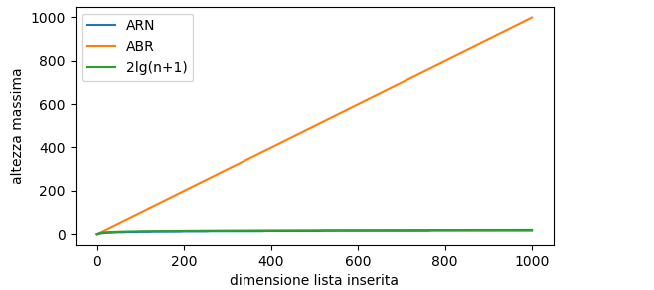
\includegraphics[scale=0.8]{img/H_ord.png}
\end{center}
\begin{table}[htbp]
\centering 
\caption{campionature delle altezze ogni 100 inserimenti\label{ordInsert}}
\begin{tabular}{l c c c c c c c c c c}
\hline\hline
\multicolumn{1}{c}{\textbf{Albero}}& \textbf{100}& \textbf{200} & \textbf{300}& \textbf{400}& \textbf{500} & \textbf{600}& \textbf{700}& \textbf{800}& \textbf{900}& \textbf{1000}\\ \hline
BR & 99 & 199 & 299 & 399 & 499 & 599 & 699 & 799 & 899 & 999\\
RN & 11 & 13 & 14 & 15 & 15 & 16 & 16 & 17 & 17 & 17\\
\hline
\end{tabular}
\end{table}
Possiamo vedere da questo grafico come le aspettative che avevamo sull'andamento dell'altezza dell'Albero Binario erano fondate, e come sperimentalmente si ha una conferma netta dell'andamento lineare dell'altezza dell'Albero Binario nel caso di inserimento di elementi in ordine crescente (o decrescente). 


Poiche la quasi totalità delle operazioni sugli Alberi Binari di Ricerca hanno un costo $O(h)$ che dipende direttamente dall'altezza $h()$ dell'albero, si ha che tutte le operazioni citate che dipendono dall'altezza costeranno, nel caso di degeneramento in una lista causato dall'inserimento in ordine, una certa quantità $O(n)$, rendendole impraticabili per alberi sbilanciati di dimensione elevata.
Questo rappresenta, ovviamente, il caso peggiore e possiamo vederne la differenza rispetto al caso medio e ottimo del grafico successivo.



Apriamo una breve parentesi sul perchè viene utilizzato un inserimento iterativo piuttosto che ricorsivo per l'Albero Binario di Ricerca: python fissa un livello massimo di ricorsioni che corrisponde a 1000, dunque negli inserimenti ordinati di una lista di dimensione superiore a 1000 elementi, la funzione di inserimento ricorsivo ha una lista di chiamate ricorsive che supera il numero da python supportato, e smette brutalmente l'inserimento lanciando una molteplici eccezioni nel tentativo di inserire ancora tale 1001-elemento. Si potrebbe aggirare il problema importando con il comando 'import sys' il modulo che permette di modificare con il comando 'sys.setrecursionlimit(100000)' il limite massimo di ricorsioni supportate. Counque accade che nell'inserimento di liste ordinate di elementi relativamente grosse $(>4000)$ al 4500-esimo elemento accade lo stesso problema riscontrato precedentemente. Si aggira il problema utilizzando una funzione iterativa per l?inserimento nell'Albero Binario di Ricerca
\begin{center}
    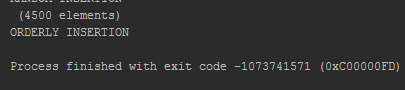
\includegraphics[scale=0.8]{img/prob.png}
\end{center}

\subsection{Inserimento Casuale}

\subsubsection{Confronti fra Altezze}
\begin{center}
    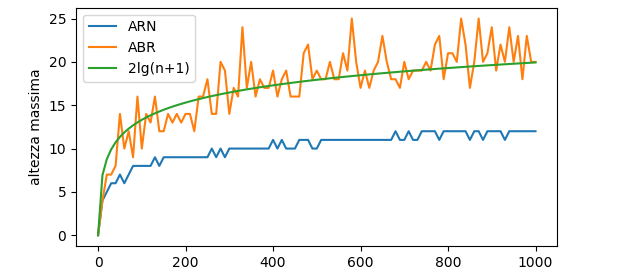
\includegraphics[scale=0.8]{img/H_disord.png}
\end{center}
\begin{table}[htbp]
\centering 
\caption{campionature delle altezze ogni 100 inserimenti\label{ordInsert}}
\begin{tabular}{l c c c c c c c c c c}
\hline\hline
\multicolumn{1}{c}{\textbf{Albero}}& \textbf{100}& \textbf{200} & \textbf{300}& \textbf{400}& \textbf{500} & \textbf{600}& \textbf{700}& \textbf{800}& \textbf{900}& \textbf{1000}\\ \hline
BR & 15 & 13 & 16 & 14 & 18 & 18 & 19 & 18 & 20 & 19\\
RN & 8 & 9 & 10 & 10 & 11 & 11 & 11 & 11 & 12 & 12\\
\hline
\end{tabular}
\end{table}
Il caso medio e migliore dell'Albero Binario di Ricerca è, appunto, quando i dati sono inseriti in ordine casuale, e dunque l'altezza dell'albero resta logaritmica $h\ = lg(n)$ e le operazioni descritte che dipendono dall'altezza avranno un costo $O(lg(n)$.
Dai grafici dell'Albero Rosso-Nero possiamo vedere come i due casi testati siano molto simili per i valori dell'altezza, e come quindi non esista un caso peggiore ed un caso migliore per questa struttura ad Albero.

\subsection{Confronto fra Tempi}

\begin{center}
    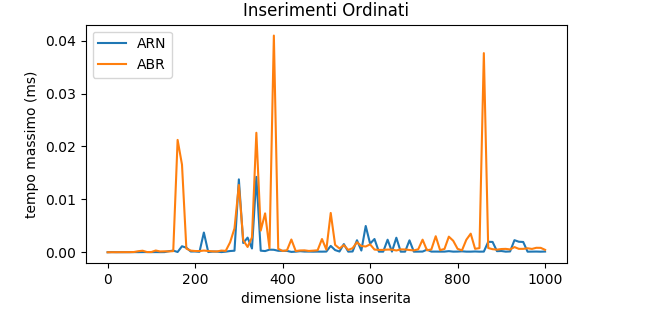
\includegraphics[scale=0.8]{img/T_ord.png}
    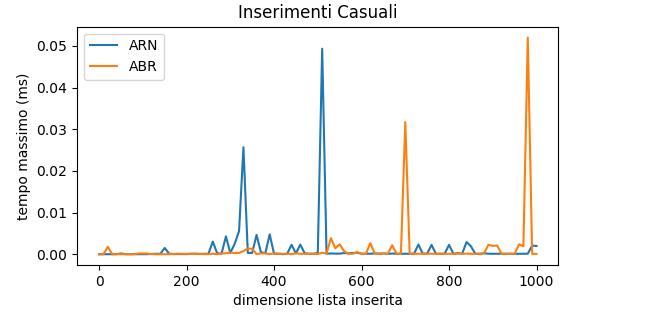
\includegraphics[scale=0.8]{img/T_disord.png}
\end{center}
Dai grafici dei tempi mi aspetto che l'albero Binario di Ricerca impieghi nettamente piu' tempo rispetto al Rosso-Nero nel caso peggiore, poichè l'albero Binario degenera in una lista e poichè il Rosso-Nero può fare al più, per ogni $insert-fix-up$ 2 rotazioni, ma vengono comunque eseguite in un tempo lineare.
si hanno però dei picchi nei grafici comportati dall'instabilita del sistema operativo, che non ci permettono di vedere affondo la dominazione nella velocità di esecuzione da parte dell'Albero Rosso-Nero.


\subsection{Lemma: altezza Rosso-Nero}

\begin{center}
    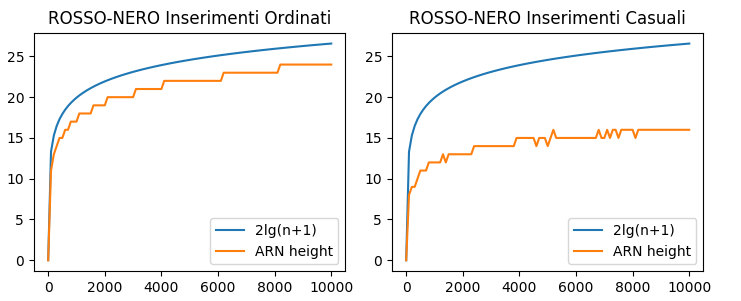
\includegraphics[scale=0.6]{img/ARN_Lemma.png}
\end{center}
Avevamo espresso precedentemente la volonta di testare la veridicità sperimentale del Lemma citato, e si è ritenuto il miglior modo di verificare il lemma quello di 'plottare' in questi due grafici sia la funzione $2 lg(n+1)$ che la funzione determinata dall'altezza massima dell'albero Rosso-Nero per numero di elementi inseriti via via crescenti.
Possiamo vedere come la funzione $2 lg(n+1)$ è sempre un limite superiore all'altezza dell'albero.
\end {document}